\newcommand\PhasenverschiebungLinks{0} % In Grad [°]
	\pgfplotsset{height=0.3\textheight}
	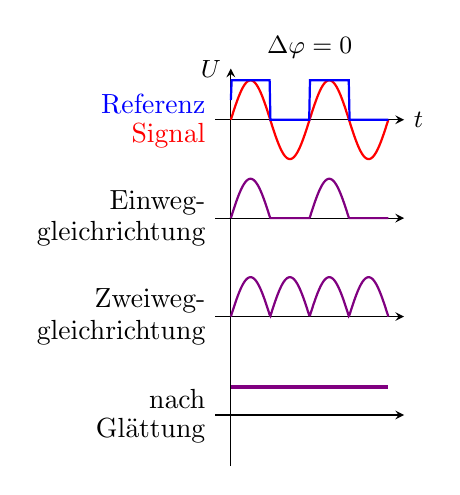
\begin{tikzpicture}[baseline]
	\begin{axis}[
	title={$\Delta \varphi = \SI{\PhasenverschiebungLinks}{\degree}$},
	x=1cm,
	y=0.5cm,
	clip=false,
	xlabel={$t$},
	ylabel={$U$},
	%xtick=\empty,
	%ytick=\empty,
	xmin=-0.2,
	xmax=2.2,
	ymin=-8.8	,
	ymax=1.3,
	xtick=\empty,
	ytick=\empty,
	axis x line=middle,
	axis y line=middle,
	scaled ticks=false,
	every axis x label/.style={
		at={(ticklabel* cs:1)},
		anchor=west,
	},
	every axis y label/.style={
		at={(ticklabel* cs:1)},
		anchor=east,
	},
	footnotesize,
	]
	\addplot [thick,red,mark=none,domain=0:2,samples=200] { sin(deg(2*pi*x)) }; % Signal
	\addplot [thick,blue,mark=none,domain=0:2,samples=200] { (sign(sin(deg(2*pi*x) + \PhasenverschiebungLinks)))/2 + 0.5 }; % Referenz mit Phasenverschiebung
	\draw [-stealth] (-0.2,-2.5) -- (2.2,-2.5);
	\addplot [thick,violet,mark=none,domain=0:2,samples=200] { sin(deg(2*pi*x))*((sign(sin(deg(2*pi*x) + \PhasenverschiebungLinks)))/2 + 0.5) - 2.5 }; % Phasenempfindliche Einweg-Gleichrichtung
	\draw [-stealth] (-0.2,-5) -- (2.2,-5);
	\addplot [thick,violet,mark=none,domain=0:2,samples=200] { sin(deg(2*pi*x))*((sign(sin(deg(2*pi*x) + \PhasenverschiebungLinks)))/2 + 0.5) + sin(deg(2*pi*x) + 180)*((sign(sin(deg(2*pi*x) + \PhasenverschiebungLinks + 180)))/2 + 0.5) - 5 }; % Phasenempfindliche Einweg-Gleichrichtung gleichgerichtet
	\draw [-stealth] (-0.2,-7.5) -- (2.2,-7.5);
	\addplot [ultra thick,violet,mark=none] coordinates { (0,{-7.5+cos(\PhasenverschiebungLinks)/sqrt(2)}) (2,{-7.5+cos(\PhasenverschiebungLinks)/sqrt(2)}) };
	\node [left] at (-0.2,+0.4) {\textcolor{blue}{Referenz}};
	\node [left] at (-0.2,-0.4) {\textcolor{red}{Signal}};
	\node [left] at (-0.2,-2.1) {Einweg-};
	\node [left] at (-0.2,-2.9) {gleichrichtung};
	\node [left] at (-0.2,-4.6) {Zweiweg-};
	\node [left] at (-0.2,-5.4) {gleichrichtung};
	\node [left] at (-0.2,-7.1) {nach};
	\node [left] at (-0.2,-7.9) {Glättung};
	\end{axis}
	\end{tikzpicture}
	% MITTE
	\newcommand\PhasenverschiebungMitte{90} % In Grad [°]
	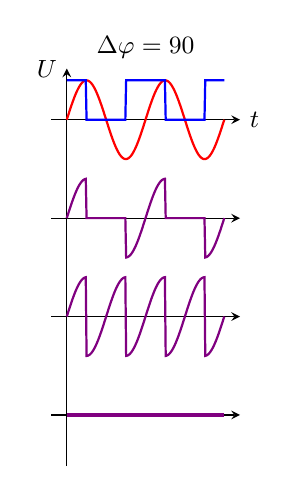
\begin{tikzpicture}[baseline]
	\begin{axis}[
	title={$\Delta \varphi = \SI{\PhasenverschiebungMitte}{\degree}$},
	x=1cm,
	y=0.5cm,
	xlabel={$t$},
	ylabel={$U$},
	%xtick=\empty,
	%ytick=\empty,
	xmin=-0.2,
	xmax=2.2,
	ymin=-8.8	,
	ymax=1.3,
	xtick=\empty,
	ytick=\empty,
	axis x line=middle,
	axis y line=middle,
	scaled ticks=false,
	every axis x label/.style={
		at={(ticklabel* cs:1)},
		anchor=west,
	},
	every axis y label/.style={
		at={(ticklabel* cs:1)},
		anchor=east,
	},
	footnotesize,
	]
	\addplot [thick,red,mark=none,domain=0:2,samples=200] { sin(deg(2*pi*x)) }; % Signal
	\addplot [thick,blue,mark=none,domain=0:2,samples=200] { (sign(sin(deg(2*pi*x) + \PhasenverschiebungMitte)))/2 + 0.5 }; % Referenz mit Phasenverschiebung
	\draw [-stealth] (-0.2,-2.5) -- (2.2,-2.5);
	\addplot [thick,violet,mark=none,domain=0:2,samples=200] { sin(deg(2*pi*x))*((sign(sin(deg(2*pi*x) + \PhasenverschiebungMitte)))/2 + 0.5) - 2.5 }; % Phasenempfindliche Einweg-Gleichrichtung
	\draw [-stealth] (-0.2,-5) -- (2.2,-5);
	\addplot [thick,violet,mark=none,domain=0:2,samples=200] { sin(deg(2*pi*x))*((sign(sin(deg(2*pi*x) + \PhasenverschiebungMitte)))/2 + 0.5) + sin(deg(2*pi*x) + 180)*((sign(sin(deg(2*pi*x) + \PhasenverschiebungMitte + 180)))/2 + 0.5) - 5 }; % Phasenempfindliche Einweg-Gleichrichtung gleichgerichtet
	\draw [-stealth] (-0.2,-7.5) -- (2.2,-7.5);
	\addplot [ultra thick,violet,mark=none] coordinates { (0,{-7.5+cos(\PhasenverschiebungMitte)/sqrt(2)}) (2,{-7.5+cos(\PhasenverschiebungMitte)/sqrt(2)}) };
	\end{axis}
	\end{tikzpicture}
	% RECHTS
	\newcommand\PhasenverschiebungRechts{180} % In Grad [°]
	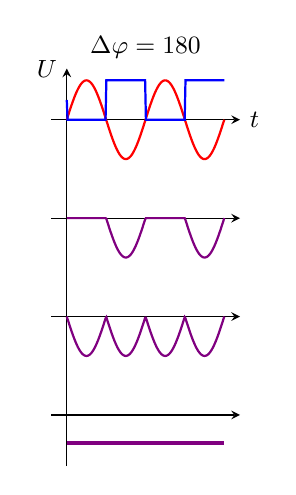
\begin{tikzpicture}[baseline]
	\begin{axis}[
	title={$\Delta \varphi = \SI{\PhasenverschiebungRechts}{\degree}$},
	x=1cm,
	y=0.5cm,
	xlabel={$t$},
	ylabel={$U$},
	%xtick=\empty,
	%ytick=\empty,
	xmin=-0.2,
	xmax=2.2,
	ymin=-8.8	,
	ymax=1.3,
	xtick=\empty,
	ytick=\empty,
	axis x line=middle,
	axis y line=middle,
	scaled ticks=false,
	every axis x label/.style={
		at={(ticklabel* cs:1)},
		anchor=west,
	},
	every axis y label/.style={
		at={(ticklabel* cs:1)},
		anchor=east,
	},
	footnotesize,
	]
	\addplot [thick,red,mark=none,domain=0:2,samples=200] { sin(deg(2*pi*x)) }; % Signal
	\addplot [thick,blue,mark=none,domain=0:2,samples=200] { (sign(sin(deg(2*pi*x) + \PhasenverschiebungRechts)))/2 + 0.5 }; % Referenz mit Phasenverschiebung
	\draw [-stealth] (-0.2,-2.5) -- (2.2,-2.5);
	\addplot [thick,violet,mark=none,domain=0:2,samples=200] { sin(deg(2*pi*x))*((sign(sin(deg(2*pi*x) + \PhasenverschiebungRechts)))/2 + 0.5) - 2.5 }; % Phasenempfindliche Einweg-Gleichrichtung
	\draw [-stealth] (-0.2,-5) -- (2.2,-5);
	\addplot [thick,violet,mark=none,domain=0:2,samples=200] { sin(deg(2*pi*x))*((sign(sin(deg(2*pi*x) + \PhasenverschiebungRechts)))/2 + 0.5) + sin(deg(2*pi*x) + 180)*((sign(sin(deg(2*pi*x) + \PhasenverschiebungRechts + 180)))/2 + 0.5) - 5 }; % Phasenempfindliche Einweg-Gleichrichtung gleichgerichtet
	\draw [-stealth] (-0.2,-7.5) -- (2.2,-7.5);
	\addplot [ultra thick,violet,mark=none] coordinates { (0,{-7.5+cos(\PhasenverschiebungRechts)/sqrt(2)}) (2,{-7.5+cos(\PhasenverschiebungRechts)/sqrt(2)}) };
	\end{axis}
\end{tikzpicture}
